\chapter{Validation}

\section{Zanghellini}

Zanghellini et al.\cite{Zanghellini04} calculate the time development of a 
one-dimensional quantum dot with two electrons using the multi-configurational 
time-dependent Hartree-Fock method (MCTDHF). This method yields excact results for 
a very large number of configurations, $\eta \to \infty$. This study would provide a 
proper benchmark for our implementation because the coupled cluster method with singles and 
doubles excitations (CCSD) is excact for $n=2$ particles. 
The harmonic oscillator potential applied in
their study had a frequency of $\omega=0.25$, used a strong laser-like field with 
maximum intensity of $E = 1$ and a laser frequency of $\Omega = 8 \omega = 2$.
Their MCTDHF scheme convergences with $\eta=15$
configurations up to the resulotion of their figures.
We are able to reproduce their results precisesly by employing the 
time-dependent coupled cluster method with singles and double excitations (TDCCSD) with 
static orbitals, using $l=20$ spin-orbitals in the basis set.

In \autoref{fig:zanghellini_fig1} we see the ground state electron density for the 
ground state wavefunction computed with CCSD. Zanghellini et al. computed the electron
density for an increasing number of configurations $\eta$ using multi-configurational
Hartree-Fock (MCHF). This figure matches the convergent electron density found by Zanghellini et al. 
as $\eta \to \infty$, in figure 1 from their article. 

\begin{figure}
    \centering
    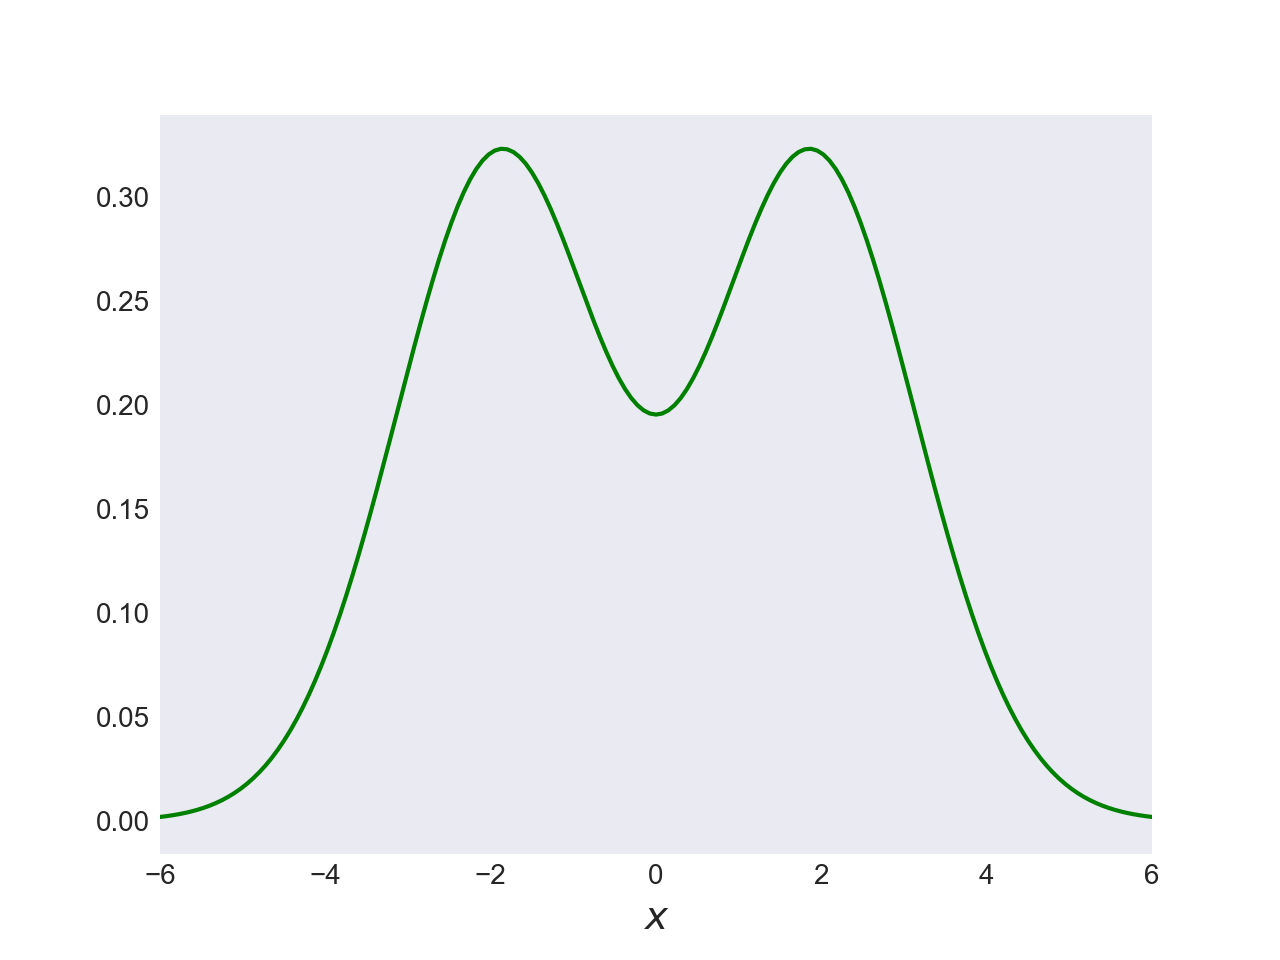
\includegraphics[width=0.75\textwidth]{results/figures/zanghellini_fig1.png}
    \caption{
        \label{fig:zanghellini_fig1}
        Electron density for the ground state wavefunction of a quantum dot with 
        $n=2$ eletrons and $l=20$ spin-orbitals in the basis set computed with
        CCSD. This plot 
        corresponds precisesly with figure 1 in Zanghellini et al.\cite{Zanghellini04}.
    }
\end{figure}

\autoref{fig:zanghellini_fig2} depicts the probability fo the system being in the ground 
state as a function of time. Here we have included both a time-dependent Hartree-Fock
computation, corresponding to a MCTDHF computation with $\eta=1$ configurations, and 
a TDCCSD computation, corresponding to MCTDHF when $\eta\to\infty$. We find that our plots
matches Zanghellin et ali's plots in their figure 2 precicely. 

\begin{figure}
    \centering
    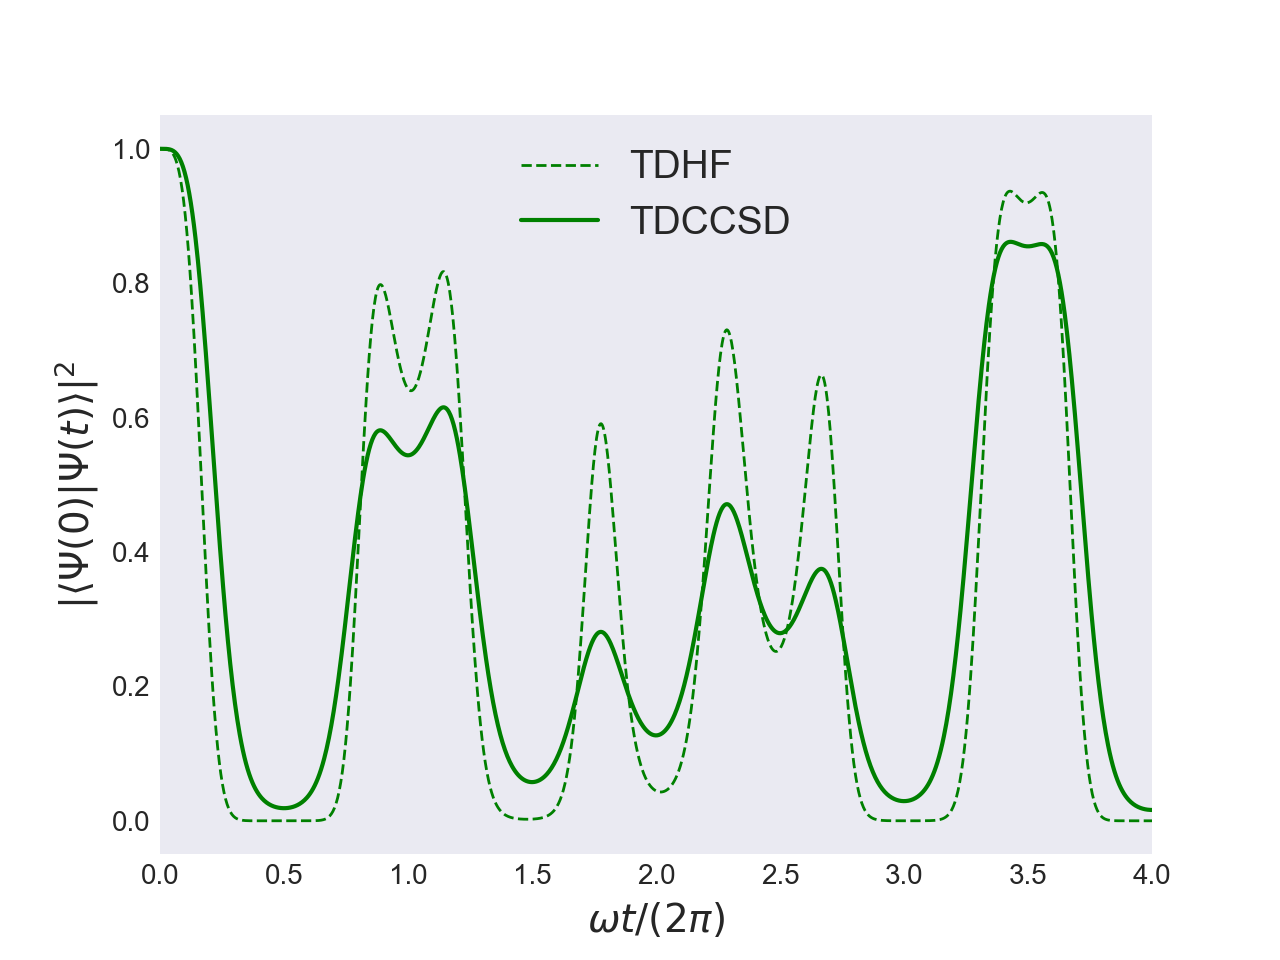
\includegraphics[width=0.75\textwidth]{results/figures/zanghellini_fig2.png}
    \caption{
        \label{fig:zanghellini_fig2}
        Probability of being in the ground state $|\braket{\Phi(0)}{\Phi(t)}|$
        using both TDHF and TDCCSD, for a one-dimensional quantum dot with $n=2$
        particles and $l=20$ spin-orbitals. This plot corresponds precisesly with 
        figure 2 in Zanghellini el al.\cite{Zanghellini04}.
    }           
\end{figure}